% MAKERSPACE RESEARCH POSTER — LaTeX source
% Inspired by the poster layout and readability advice in UNLV's
% "Poster Design Workshop Slides" (especially slides 15, 30, 34, 36, 39).
% Compile with: pdflatex main.tex
% Upload Article1.png, Article2.png, Article3.png, Article4.png in the same directory.
% Upload unlv_engineering.png in the same Overleaf directory as main.tex.
% A stand-in wordmark appears if that PNG is missing; replace with official logo.
\documentclass[final]{article}
\usepackage[paperwidth=48in,paperheight=36in,margin=0in]{geometry}
\usepackage[T1]{fontenc}
\usepackage{lmodern}
\usepackage{tikz}
\usetikzlibrary{arrows.meta,positioning,shapes.geometric}
\usepackage{xcolor}
\usepackage{ragged2e}
\usepackage{graphicx}
\usepackage{eso-pic}
\pagestyle{empty}
\setlength{\parindent}{0pt}
\definecolor{unlvred}{HTML}{A60B22}
\definecolor{headerred}{HTML}{C52B3E}
\definecolor{maroon}{HTML}{280910}
\definecolor{ink}{HTML}{F5F7FA}
\definecolor{muted}{HTML}{B9C2CC}
\definecolor{palebg}{HTML}{080C12}
\definecolor{palered}{HTML}{251721}
\definecolor{linegray}{HTML}{3F4A59}
\definecolor{lightblue}{HTML}{152A3F}
\definecolor{panelbg}{HTML}{151B24}
\newcommand{\bodyfont}{\fontsize{26}{34}\selectfont}
\newcommand{\smallfont}{\fontsize{22}{28}\selectfont}
\newcommand{\sectionfont}{\fontsize{32}{37}\bfseries\selectfont}
\newcommand{\posterbox}[6]{%
  % x, top-y, width, height, title, content
  \filldraw[fill=panelbg,draw=linegray,line width=1.7pt,rounded corners=15pt]
     (#1,#2) rectangle ++(#3,-#4);
  \fill[unlvred,rounded corners=12pt] (#1,#2) rectangle ++(#3,-0.76);
  \node[anchor=west,text=white] at ({#1+0.35},{#2-0.38}) {\sectionfont #5};
  \node[anchor=north west,inner sep=0pt,text width=\dimexpr#3in-0.7in\relax,
        align=left] at ({#1+0.36},{#2-1.05}) {\bodyfont\color{ink}#6};
}
\begin{document}
\AddToShipoutPictureBG*{\AtPageLowerLeft{
\begin{tikzpicture}[x=1in,y=1in]
  \begin{scope}
    \fill[palebg] (-0.1,-0.1) rectangle (48.1,36.15);
    % HEADER: reduced height, richer slightly darkened red, dark typography.
    \fill[headerred] (-0.1,31.9) rectangle (48.1,36.15);
    % Narrow dark-red accent at the bottom; no white/gray rails around header.
    \fill[headerred!80!black] (-0.1,31.9) rectangle (48.1,31.98);
    \draw[black!45,line width=2pt] (13.5,32.48) -- (13.5,35.35);
    \draw[black!45,line width=2pt] (36.6,32.48) -- (36.6,35.35);
    % A deliberate header logo region. The image is supplied by the user in Overleaf.
    % If PNG is surrounded by blank pixels, edit trim values in this line.
    \IfFileExists{unlv_engineering.png}{%
      \node[anchor=center,inner sep=0pt] at (6.6,33.98)
        {
\includegraphics[width=12.6in,height=3.85in,keepaspectratio,
         trim=0 0 0 0,clip]{unlv_engineering.png}};
    }{%
      % Typographic approximation ONLY for local preview until official PNG is uploaded.
      \node[align=center,text=black,inner sep=0pt] at (6.6,34.02)
        {{\fontsize{142}{145}\selectfont UNLV}\\[0.06em]
         {\fontsize{31}{36}\selectfont HOWARD R. HUGHES}\\
         {\fontsize{31}{36}\selectfont COLLEGE OF ENGINEERING}};
    }
    \node[anchor=center,text=black] at (25.15,34.60)
      {\fontsize{90}{98}\bfseries\selectfont M.A.C};
    \node[anchor=center,text=black] at (25.15,33.10)
      {\fontsize{34}{41}\bfseries\selectfont Makerspace Access Control};
    % Accent under project name, different from title bar
    \fill[black!70,rounded corners=5pt] (21.55,32.53) rectangle (28.75,32.59);
    % Custom M.A.C gear + lock logo, slightly smaller to suit the shorter banner.
    \begin{scope}[shift={(42.2,33.93)},scale=0.76]
       \foreach \a in {0,30,...,330} {
         \begin{scope}[rotate=\a]
           \fill[black,rounded corners=3pt] (-0.25,1.17) rectangle (0.25,1.73);
         \end{scope}
       }
       \filldraw[fill=headerred,draw=black,line width=7pt] (0,0) circle (1.30);
       \draw[black,line width=4pt] (0,0) circle (0.97);
       \draw[black,line width=8pt,rounded corners=8pt]
          (-0.44,-0.05) -- (-0.44,0.42) arc[start angle=180,end angle=0,radius=0.44] -- (0.44,-0.05);
       \fill[black,rounded corners=7pt] (-0.61,-0.52) rectangle (0.61,0.10);
       \fill[headerred] (0,-0.18) circle (0.10);
       \draw[headerred,line width=4pt] (0,-0.22) -- (0,-0.36);
       \draw[black,line width=5pt] (1.12,1.16) arc[start angle=42,end angle=77,radius=1.62];
       \draw[black,line width=5pt] (1.30,1.36) arc[start angle=43,end angle=77,radius=2.02];
    \end{scope}

    % Scale all poster panels/diagrams vertically into the area gained from header.
    % This leaves the existing lower layout/line spacing unchanged in width.
    \begin{scope}[yscale=1.04]
    % Left column — grounded in DP II project portfolio
    % Background - purposely uses the full height, with readable separated issues
    \filldraw[fill=panelbg,draw=linegray,line width=1.7pt,rounded corners=15pt]
       (0.8,29.9) rectangle (14.3,21.9);
    \fill[unlvred,rounded corners=12pt] (0.8,29.9) rectangle ++(13.5,-0.76);
    \node[anchor=west,text=white] at (1.15,29.52) {\sectionfont Background};
    \node[anchor=north west,text width=12.5in,align=left,inner sep=0pt]
      at (1.22,28.7) {{\fontsize{29}{36}\bfseries\selectfont\color{white}
        MAC connects machine access to user certifications, helping prevent
        unauthorized use while simplifying Makerspace supervision.}};
    % Divider directly separates the overview from the numbered background points.
    \draw[unlvred,line width=1.8pt] (1.24,27.30) -- (13.82,27.30);
    \tikzset{issueicon/.style={draw=unlvred,fill=palered,line width=2pt,circle,
             minimum size=0.60in,text=white,font=\fontsize{21}{25}\bfseries\selectfont}}
    \node[issueicon] at (1.72,26.10) {1};
    \node[anchor=north west,text width=11.15in,inner sep=0pt,align=left] at (2.3,26.40)
      {{\fontsize{24}{30}\selectfont\color{ink}
        \textbf{Unauthorized equipment use:} Machines can be accessed without required training or permission.}};
    \node[issueicon] at (1.72,24.93) {2};
    \node[anchor=north west,text width=11.15in,inner sep=0pt,align=left] at (2.3,25.23)
      {{\fontsize{24}{30}\selectfont\color{ink}
        \textbf{Supervisor workload:} Staff must manually verify credentials and unlock equipment.}};
    \node[issueicon] at (1.72,23.76) {3};
    \node[anchor=north west,text width=11.15in,inner sep=0pt,align=left] at (2.3,24.06)
      {{\fontsize{24}{30}\selectfont\color{ink}
        \textbf{Fragmented records:} Local documents make authorization difficult to verify consistently.}};
    \node[issueicon] at (1.72,22.59) {4};
    \node[anchor=north west,text width=11.15in,inner sep=0pt,align=left] at (2.3,22.89)
      {{\fontsize{24}{30}\selectfont\color{ink}
        \textbf{Limited usage tracking:} Machine activity is difficult to audit for maintenance or misuse.}};
    % MVP Features: independent title and description nodes avoid tight line spacing.
    \filldraw[fill=panelbg,draw=linegray,line width=1.7pt,rounded corners=15pt]
       (0.8,21.1) rectangle (14.3,15.3);
    \fill[unlvred,rounded corners=12pt] (0.8,21.1) rectangle ++(13.5,-0.76);
    \node[anchor=west,text=white] at (1.15,20.72) {\sectionfont MVP Features};
    \tikzset{mvpnum/.style={draw=unlvred,fill=palered,line width=1.7pt,circle,
         minimum size=0.63in,inner sep=0pt,text=white,font=\fontsize{23}{28}\bfseries\selectfont}}
    % Feature 1: circle at row center; lines separated by 0.50 in.
    \node[mvpnum] at (1.66,19.69) {1};
    \node[anchor=west,inner sep=0pt,text=white,
          font=\fontsize{24}{29}\bfseries\selectfont]
       at (2.39,19.94) {Check-in};
    \node[anchor=west,inner sep=0pt,text=ink,
          font=\fontsize{19}{24}\selectfont]
       at (2.39,19.44) {RebelCard lookup and NSHE ID entry};
    \draw[linegray,line width=0.8pt] (1.35,19.06) -- (13.75,19.06);
    % Feature 2: circle at row center; lines separated by 0.50 in.
    \node[mvpnum] at (1.66,18.46) {2};
    \node[anchor=west,inner sep=0pt,text=white,
          font=\fontsize{24}{29}\bfseries\selectfont]
       at (2.39,18.71) {Results page};
    \node[anchor=west,inner sep=0pt,text=ink,
          font=\fontsize{19}{24}\selectfont]
       at (2.39,18.21) {Show certifications, eligible machines, and restrictions};
    \draw[linegray,line width=0.8pt] (1.35,17.83) -- (13.75,17.83);
    % Feature 3: circle at row center; lines separated by 0.50 in.
    \node[mvpnum] at (1.66,17.23) {3};
    \node[anchor=west,inner sep=0pt,text=white,
          font=\fontsize{24}{29}\bfseries\selectfont]
       at (2.39,17.48) {Administration};
    \node[anchor=west,inner sep=0pt,text=ink,
          font=\fontsize{19}{24}\selectfont]
       at (2.39,16.98) {Manage users, certifications, and machine requirements};
    \draw[linegray,line width=0.8pt] (1.35,16.60) -- (13.75,16.60);
    % Feature 4: circle at row center; lines separated by 0.50 in.
    \node[mvpnum] at (1.66,16.00) {4};
    \node[anchor=west,inner sep=0pt,text=white,
          font=\fontsize{24}{29}\bfseries\selectfont]
       at (2.39,16.25) {Device communication};
    \node[anchor=west,inner sep=0pt,text=ink,
          font=\fontsize{19}{24}\selectfont]
       at (2.39,15.75) {Backend-to-ESP8266 commands for future machine control};
    % Implementation Stack: concise text list first, distinct diagram underneath.
    \filldraw[fill=panelbg,draw=linegray,line width=1.7pt,rounded corners=15pt]
      (0.8,14.4) rectangle (14.3,1.0);
    \fill[unlvred,rounded corners=12pt] (0.8,14.4) rectangle ++(13.5,-0.76);
    \node[anchor=west,text=white] at (1.15,14.02) {\sectionfont Implementation Stack};
    % One readable row per technology, with a clear bold label.
    \node[anchor=west,text=ink,font=\fontsize{23}{29}\selectfont] at (1.25,12.72)
      {\textbf{Frontend:} React / Remix + TypeScript};
    \node[anchor=west,text=ink,font=\fontsize{23}{29}\selectfont] at (1.25,11.82)
      {\textbf{Backend:} Node.js + TypeScript};
    \node[anchor=west,text=ink,font=\fontsize{23}{29}\selectfont] at (1.25,10.92)
      {\textbf{Database:} PostgreSQL + Prisma ORM};
    \node[anchor=west,text=ink,font=\fontsize{23}{29}\selectfont] at (1.25,10.02)
      {\textbf{Satellite:} ESP8266, Wi-Fi, HTTP / JSON};
    \node[anchor=west,text=ink,font=\fontsize{23}{29}\selectfont] at (1.25,9.12)
      {\textbf{Deployment:} Docker + Ubuntu VPS (Portainer)};
    \node[anchor=west,text=ink,font=\fontsize{23}{29}\selectfont] at (1.25,8.22)
      {\textbf{Testing:} Vitest; end-to-end checks in progress};

    \draw[linegray,line width=1.2pt] (1.25,7.45) -- (13.85,7.45);
    \node[anchor=west,text=ink,font=\fontsize{23}{29}\bfseries\selectfont]
      at (1.25,6.76) {How the components connect};

    % Supporting schematic, not a replacement for the text list.
    \tikzset{smallstack/.style={draw=white,fill=lightblue,
                 rounded corners=10pt,line width=2.2pt,
                 minimum width=3.5in,minimum height=1.22in,
                 align=center,text=white,font=\fontsize{19}{25}\selectfont},
              smallarrow/.style={-Latex,draw=white!85,line width=2.5pt}}
    \node[smallstack] (s-ui) at (3.05,5.17) {Kiosk / Admin\\\fontsize{16}{21}\selectfont React + Remix};
    \node[smallstack] (s-api) at (7.55,5.17) {Backend API\\\fontsize{16}{21}\selectfont Node.js};
    \node[smallstack] (s-db) at (12.0,5.17) {Database\\\fontsize{16}{21}\selectfont PostgreSQL};
    \node[smallstack,minimum width=4.0in] (s-esp) at (7.55,2.93)
      {ESP8266 Satellite\\\fontsize{16}{21}\selectfont HTTP status + commands};
    \draw[smallarrow] (s-ui.east) -- (s-api.west);
    \draw[smallarrow] (s-api.east) -- (s-db.west);
    \draw[smallarrow] (s-api.south) -- (s-esp.north);
    \node[anchor=center,text=muted,font=\fontsize{16}{21}\selectfont]
      at (7.55,1.57) {Physical machine activation: future integration};
    % CENTER COLUMN: original prototype screens and architecture.
    % All four Article images are bundled in the Overleaf ZIP.
    \filldraw[fill=panelbg,draw=linegray,line width=1.7pt,rounded corners=15pt]
       (15.1,29.9) rectangle (33.35,1.6);
    \fill[unlvred,rounded corners=12pt] (15.1,29.9) rectangle ++(18.25,-0.76);
    \node[anchor=west,text=white] at (15.48,29.51)
       {\sectionfont System Architecture and Demonstration};

        % Architecture illustration without a repeated inner title.
    \filldraw[fill=white,draw=linegray,line width=1.2pt,rounded corners=12pt]
       (15.75,28.35) rectangle (32.70,21.55);
    \node[anchor=center,inner sep=0pt] at (24.22,24.98)
      {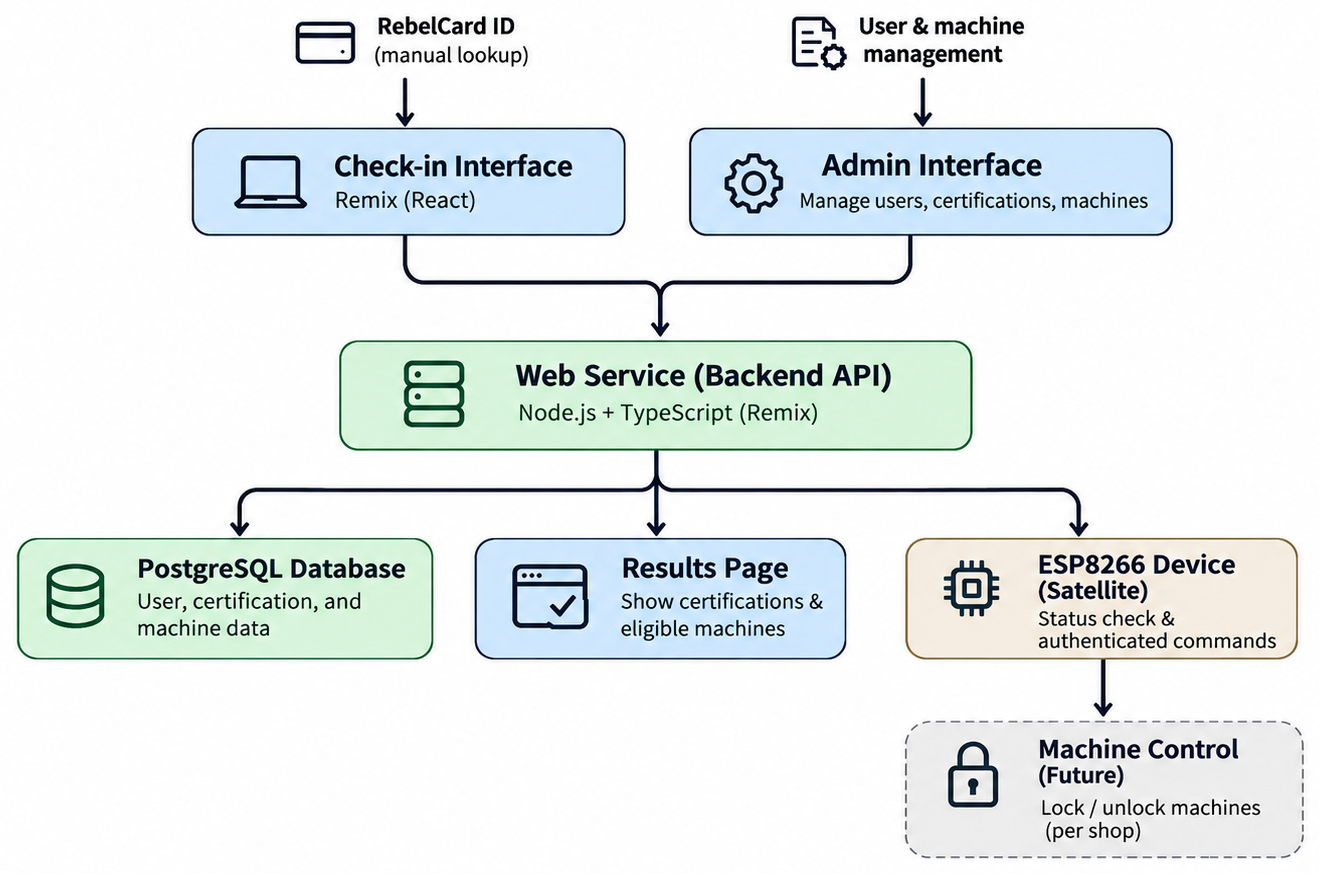
\includegraphics[width=16.78in,height=6.42in,keepaspectratio]{Article1_cropped.png}};
    \node[anchor=west,text=ink,font=\fontsize{18}{23}\selectfont]
       at (15.86,21.06) {\textbf{Figure 1.} Current backend, database, results, admin, and ESP8266 communication flow.};

    % Two balanced screenshot cards: vertically stacked title, image and caption.
    % The results screenshot is portrait/square and should not sit in a very wide card.
    \filldraw[fill=lightblue,draw=white,line width=2.2pt,rounded corners=11pt]
       (15.74,20.15) rectangle (24.13,10.75);
    \filldraw[fill=lightblue,draw=white,line width=2.2pt,rounded corners=11pt]
       (24.33,20.15) rectangle (32.72,10.75);

    % Left card heading + white divider.
    \node[anchor=west,text=unlvred,font=\fontsize{26}{32}\bfseries\selectfont]
       at (16.08,19.63) {Student Check-In};
    \draw[line width=1.4pt,white] (16.08,19.26) -- (23.79,19.26);
    % Delicate white border framing the enlarged check-in screenshot.
    \filldraw[fill=black,draw=white,line width=1.15pt]
       (16.29,12.00) rectangle (23.58,18.98);
    \node[anchor=center,inner sep=0pt] at (19.935,15.49)
       {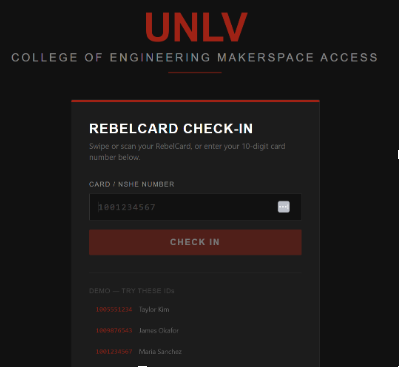
\includegraphics[width=7.24in,height=6.93in,keepaspectratio]{Article2.png}};
    \node[anchor=north west,text width=7.63in,inner sep=0pt,align=left]
       at (16.14,11.57) {{\fontsize{18}{24}\selectfont\color{ink}RebelCard or ID entry initiates student verification.}};

    % Right card heading + white divider.
    \node[anchor=west,text=unlvred,font=\fontsize{26}{32}\bfseries\selectfont]
       at (24.65,19.63) {Machine Eligibility Results};
    \draw[line width=1.4pt,white] (24.65,19.26) -- (32.39,19.26);
    % Square screenshot uses the available height without wide blank side margins.
    \filldraw[fill=black,draw=white,line width=1.15pt]
       (25.00,12.00) rectangle (32.06,18.98);
    \node[anchor=center,inner sep=0pt] at (28.53,15.49)
       {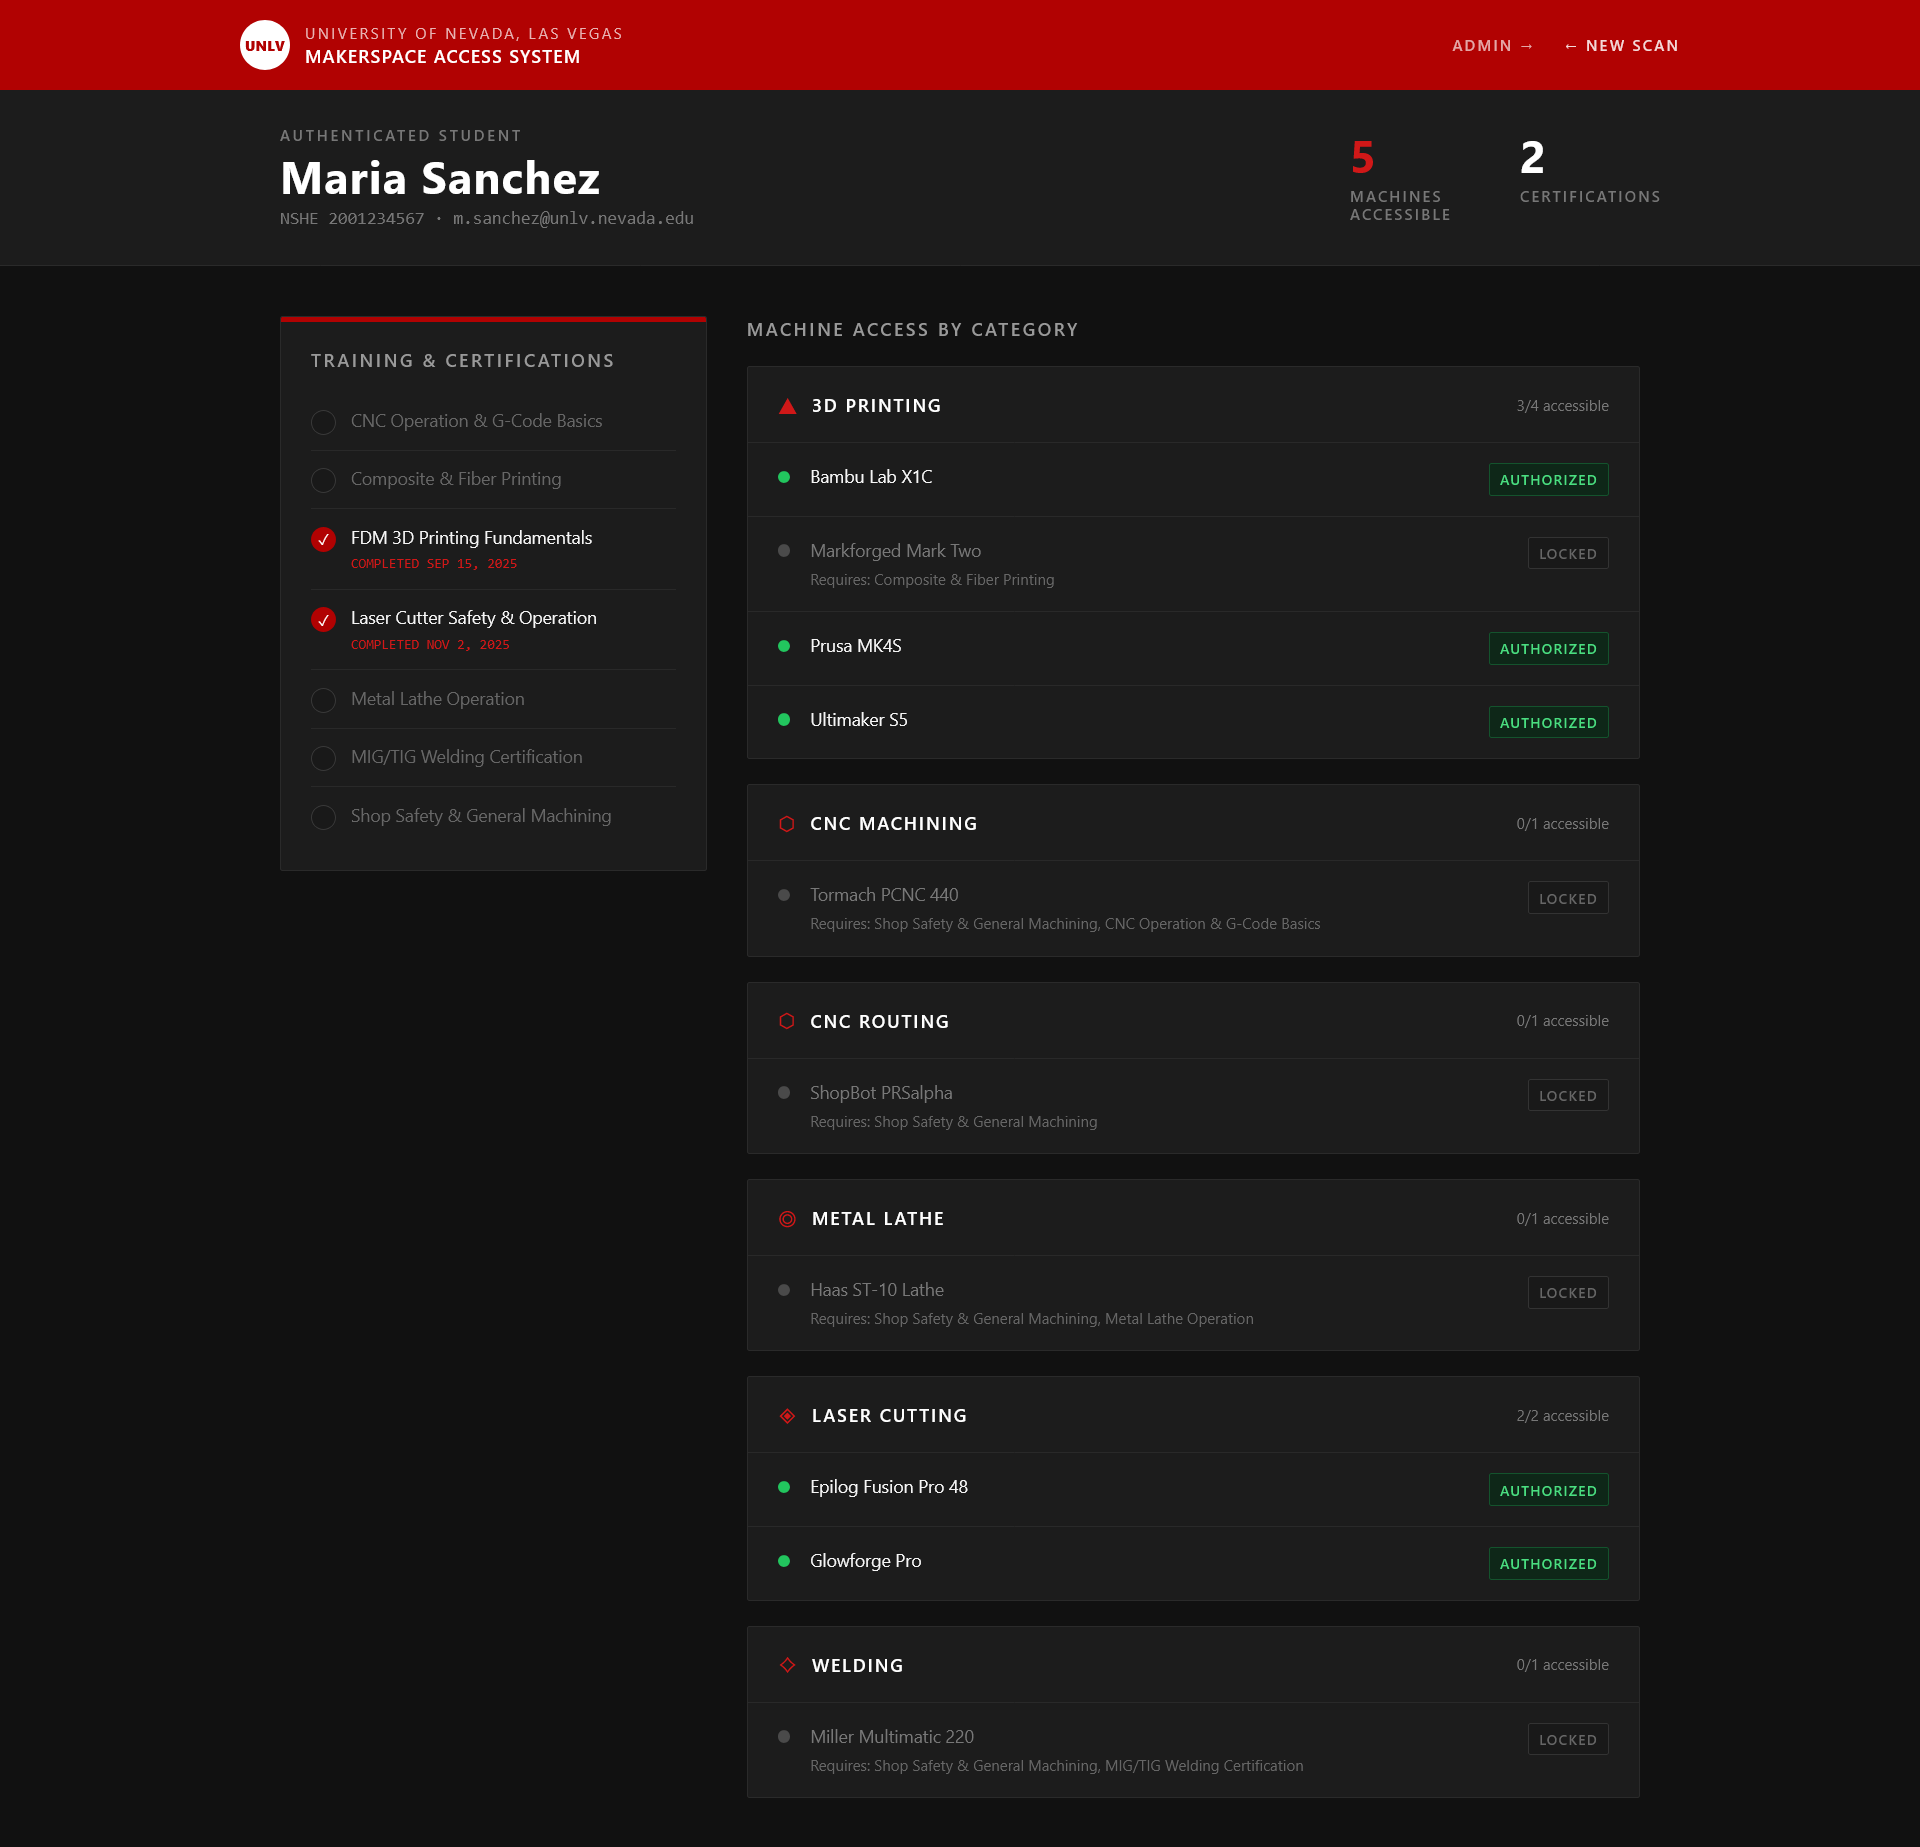
\includegraphics[width=7.01in,height=6.93in,keepaspectratio]{Article4.png}};
    \node[anchor=north west,text width=7.61in,inner sep=0pt,align=left]
       at (24.71,11.57) {{\fontsize{18}{24}\selectfont\color{ink}Certifications determine accessible and locked machines.}};

    % Admin interface: image on left with design summary on right.
    \filldraw[fill=lightblue,draw=white,line width=2.2pt,rounded corners=11pt]
       (15.74,10.20) rectangle (32.72,2.18);
    \node[anchor=west,text=unlvred,font=\fontsize{25}{31}\bfseries\selectfont]
       at (16.07,9.72) {Administrative Management Console};
    \draw[line width=1.4pt,white] (16.07,9.37) -- (32.36,9.37);
    % Keep screenshot inside a fine white outline and toward left edge.
    \filldraw[fill=black,draw=white,line width=1.3pt]
       (16.09,3.10) rectangle (24.20,8.99);
    \node[anchor=center,inner sep=0pt] at (20.145,6.045)
       {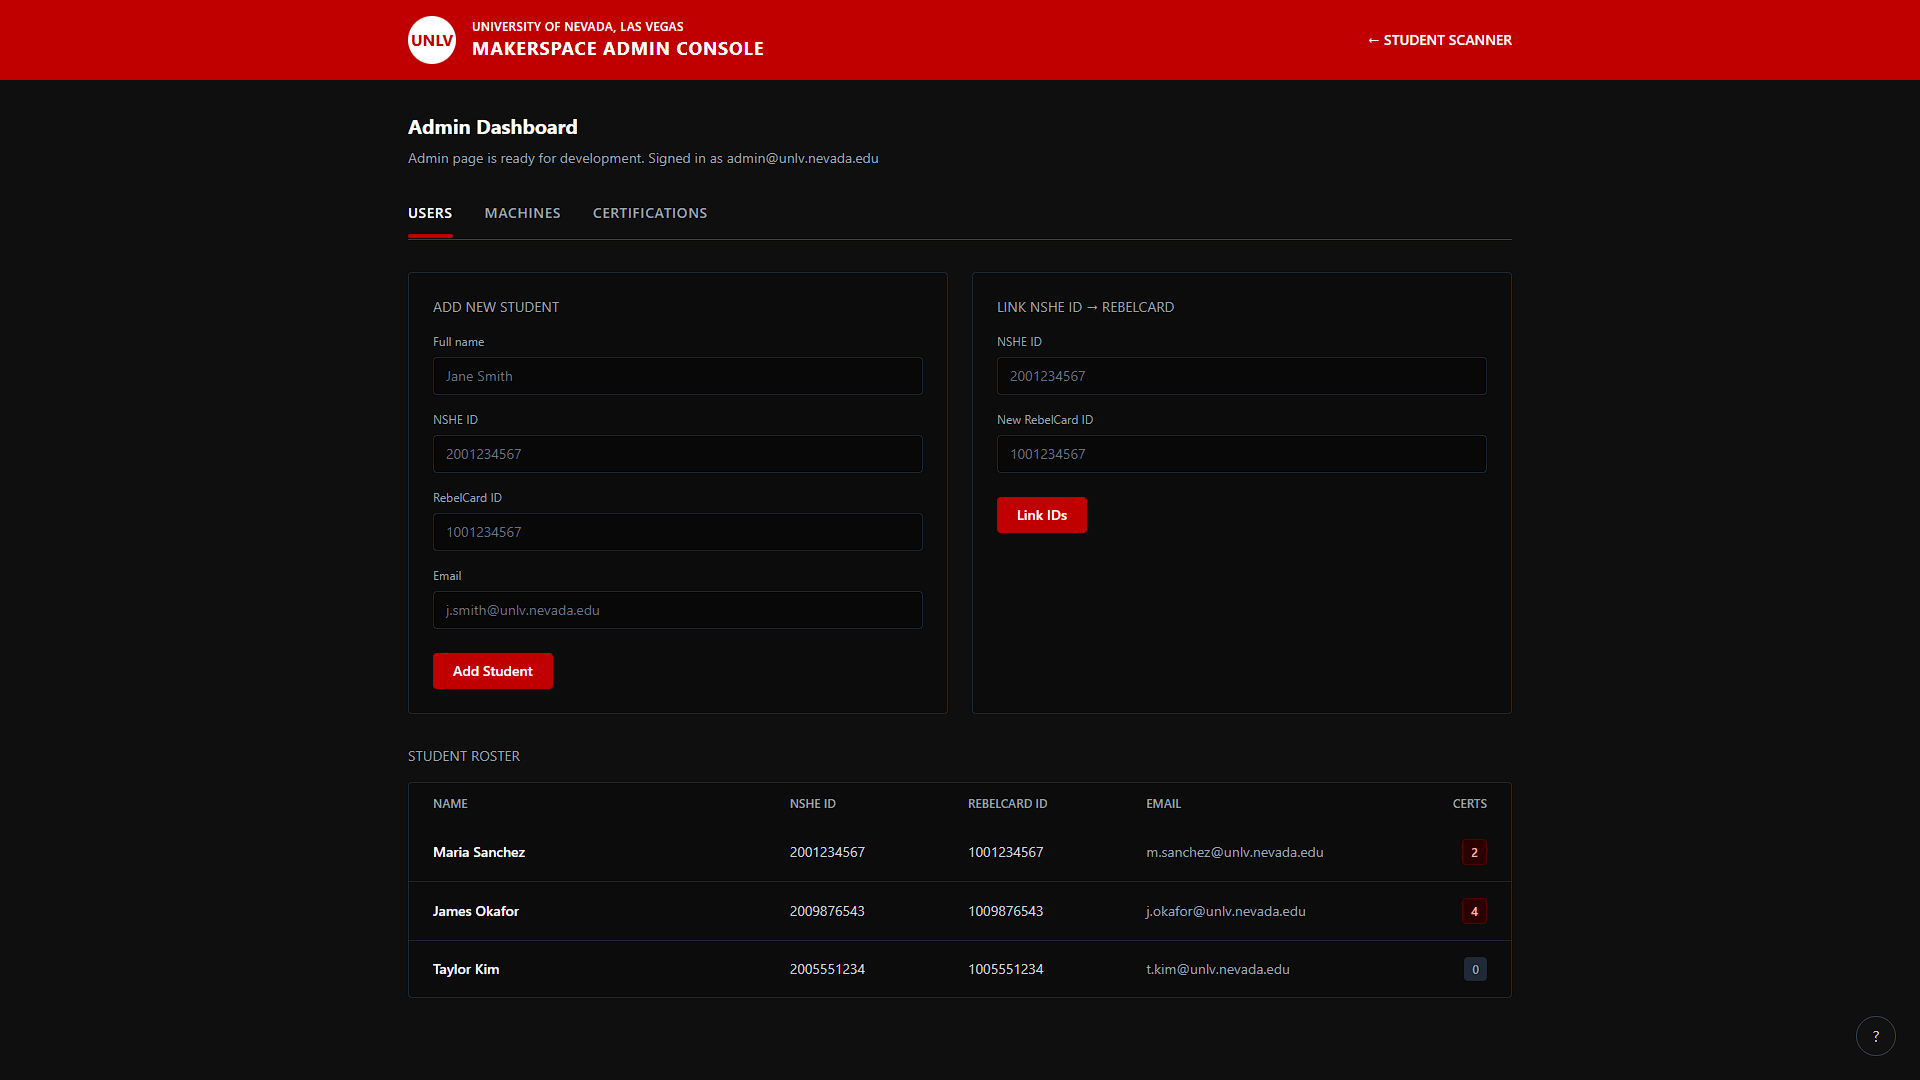
\includegraphics[width=8.05in,height=5.82in,keepaspectratio]{Article3.png}};
    % Explanation alongside the screenshot: design capabilities, not claims of completed activation.
    \node[anchor=north west,text width=7.46in,inner sep=0pt,align=left]
       at (24.62,8.91) {{\fontsize{25}{31}\bfseries\selectfont\color{white} Design Summary}};
    \draw[white,line width=1.0pt] (24.62,8.39) -- (32.20,8.39);
    % Four concise design points with independent title and description baselines.
    \node[anchor=north west,text width=7.40in,inner sep=0pt,align=left]
       at (24.62,8.10) {{\fontsize{19}{24}\bfseries\selectfont\color{white}Centralized records}};
    \node[anchor=north west,text width=7.40in,inner sep=0pt,align=left]
       at (24.62,7.70) {{\fontsize{17}{23}\selectfont\color{ink}Brings student profiles, certifications, and machine records into one central database.}};

    \node[anchor=north west,text width=7.40in,inner sep=0pt,align=left]
       at (24.62,6.83) {{\fontsize{19}{24}\bfseries\selectfont\color{white}Role-based administration}};
    \node[anchor=north west,text width=7.40in,inner sep=0pt,align=left]
       at (24.62,6.43) {{\fontsize{17}{23}\selectfont\color{ink}Gives authorized staff a dedicated interface to maintain users, certifications, and machine information.}};

    \node[anchor=north west,text width=7.40in,inner sep=0pt,align=left]
       at (24.62,5.56) {{\fontsize{19}{24}\bfseries\selectfont\color{white}Machine eligibility}};
    \node[anchor=north west,text width=7.40in,inner sep=0pt,align=left]
       at (24.62,5.16) {{\fontsize{17}{23}\selectfont\color{ink}Identifies machines each student is qualified to use, with machine listings and access status.}};

    \node[anchor=north west,text width=7.40in,inner sep=0pt,align=left]
       at (24.62,4.20) {{\fontsize{19}{24}\bfseries\selectfont\color{white}Overall system design}};
    \node[anchor=north west,text width=7.40in,inner sep=0pt,align=left]
       at (24.62,3.80) {{\fontsize{17}{23}\selectfont\color{ink}Connects student check-in, eligibility results, administration, and ESP8266 communication in one system.}};
    % Right column — evidence and careful MVP status distinctions
    % Components: four balanced rows with independently positioned text.
    % Number circles are centered between the title and description lines.
    \filldraw[fill=panelbg,draw=linegray,line width=1.7pt,rounded corners=15pt]
       (34.1,29.9) rectangle (47.2,21.5);
    \fill[unlvred,rounded corners=12pt] (34.1,29.9) rectangle ++(13.1,-0.76);
    \node[anchor=west,text=white] at (34.45,29.52) {\sectionfont Components};
    \tikzset{protoicon/.style={draw=unlvred,fill=palered,line width=1.7pt,circle,
       minimum size=0.68in,inner sep=0pt,text=white,
       font=\fontsize{23}{28}\bfseries\selectfont}}
    % Thin dividers maintain visual separation without adding extra headings.
    \foreach \yy in {27.015,25.145,23.275}{
       \draw[linegray,line width=0.8pt] (34.78,\yy) -- (46.55,\yy);
    }
    % Row 1
    \node[protoicon] at (35.12,27.95) {1};
    \node[anchor=west,inner sep=0pt,text=white,
          font=\fontsize{27}{33}\bfseries\selectfont]
       at (35.95,28.27) {Check-in System};
    \node[anchor=west,inner sep=0pt,text=ink,
          font=\fontsize{22}{28}\selectfont]
       at (35.95,27.61) {RebelCard ID lookup connected to PostgreSQL.};
    % Row 2
    \node[protoicon] at (35.12,26.08) {2};
    \node[anchor=west,inner sep=0pt,text=white,
          font=\fontsize{27}{33}\bfseries\selectfont]
       at (35.95,26.40) {Results Page};
    \node[anchor=west,inner sep=0pt,text=ink,
          font=\fontsize{22}{28}\selectfont]
       at (35.95,25.74) {Shows certifications and eligible machines.};
    % Row 3
    \node[protoicon] at (35.12,24.21) {3};
    \node[anchor=west,inner sep=0pt,text=white,
          font=\fontsize{27}{33}\bfseries\selectfont]
       at (35.95,24.53) {Admin Interface};
    \node[anchor=west,inner sep=0pt,text=ink,
          font=\fontsize{22}{28}\selectfont]
       at (35.95,23.87) {Role-based access and initial admin tools implemented.};
    % Row 4
    \node[protoicon] at (35.12,22.34) {4};
    \node[anchor=west,inner sep=0pt,text=white,
          font=\fontsize{27}{33}\bfseries\selectfont]
       at (35.95,22.66) {ESP8266 Communication};
    \node[anchor=west,inner sep=0pt,text=ink,
          font=\fontsize{22}{28}\selectfont]
       at (35.95,22.00) {Status and authenticated commands supported.};
    % Evidence / Testing: matched two-column layout with a vertical workflow.
    % All content fits inside the original panel; no image placeholders.
    \filldraw[fill=panelbg,draw=linegray,line width=1.7pt,rounded corners=15pt]
       (34.1,20.7) rectangle (47.2,13.7);
    \fill[unlvred,rounded corners=12pt] (34.1,20.7) rectangle ++(13.1,-0.76);
    \node[anchor=west,text=white] at (34.45,20.32)
       {\sectionfont Evidence / Testing};

    % Left: compact evidence descriptions and simple bullets.
    \node[anchor=west,text=headerred,font=\fontsize{25}{30}\bfseries\selectfont]
       at (34.55,19.52) {Continuous Integration (CI)};
    \draw[white!75,line width=1.1pt] (34.56,19.16) -- (40.35,19.16);
    \node[anchor=north west,inner sep=0pt,text width=5.65in,align=left]
       at (34.58,18.96) {\fontsize{19}{25}\selectfont\color{ink}
       Automated checks validate code changes before they are merged.};
    \node[anchor=west,text=headerred,font=\fontsize{20}{25}\selectfont]
       at (34.68,18.02) {$\bullet$};
    \node[anchor=west,text=ink,font=\fontsize{19}{25}\selectfont]
       at (35.02,18.02) {Run on each pull request.};
    \node[anchor=west,text=headerred,font=\fontsize{20}{25}\selectfont]
       at (34.68,17.60) {$\bullet$};
    \node[anchor=west,text=ink,font=\fontsize{19}{25}\selectfont]
       at (35.02,17.60) {Fix failed checks before merging.};

    \node[anchor=west,text=headerred,font=\fontsize{25}{30}\bfseries\selectfont]
       at (34.55,16.92) {Vitest Unit Tests};
    \draw[white!75,line width=1.1pt] (34.56,16.56) -- (40.35,16.56);
    \node[anchor=north west,inner sep=0pt,text width=5.65in,align=left]
       at (34.58,16.34) {\fontsize{19}{25}\selectfont\color{ink}
       Tests validate API responses and errors.};
    \node[anchor=west,text=headerred,font=\fontsize{20}{25}\selectfont]
       at (34.68,15.38) {$\bullet$};
    \node[anchor=west,text=ink,font=\fontsize{18}{24}\selectfont]
       at (35.02,15.38) {Run tests locally with Vitest.};
    \node[anchor=west,text=headerred,font=\fontsize{20}{25}\selectfont]
       at (34.68,14.96) {$\bullet$};
    \node[anchor=west,text=ink,font=\fontsize{18}{24}\selectfont]
       at (35.02,14.96) {Confirm tests also pass in CI.};

    % Vertical separator: same thin-rule treatment as the center column.
    \draw[linegray,line width=1.4pt] (40.70,14.13) -- (40.70,19.58);
    % Right: minimal vertical process; all boxes are TikZ shapes (not images).
    \node[anchor=west,text=headerred,font=\fontsize{25}{30}\bfseries\selectfont]
       at (41.04,19.52) {Testing Workflow};
    \draw[white!75,line width=1.1pt] (41.04,19.16) -- (46.73,19.16);

    \tikzset{verifybox/.style={draw=white!55,fill=panelbg,
          rounded corners=6pt,line width=1.25pt,
          minimum width=4.25in,minimum height=0.65in,
          inner sep=3pt,align=center,text=ink,
          font=\fontsize{18}{23}\selectfont},
          verifyend/.style={draw=white!60,fill=panelbg,
          rounded corners=6pt,line width=1.3pt,
          minimum width=2.45in,minimum height=0.62in,
          inner sep=3pt,align=center,text=ink,
          font=\fontsize{17}{21}\selectfont},
          verifyarrow/.style={-Latex,draw=white!85,line width=1.65pt}}
    \node[verifybox] (v-pr) at (43.85,18.49) {Feature Branch / Pull Request};
    \node[verifybox] (v-ci) at (43.85,17.32) {CI Checks + Vitest};
    \node[diamond,draw=white,fill=lightblue,
          line width=2.2pt,aspect=2.6,
          minimum width=3.15in,minimum height=0.95in,
          inner sep=2pt,align=center,text=ink,
          font=\fontsize{18}{22}\bfseries\selectfont]
          (v-decision) at (43.85,16.08) {All checks pass?};
    \node[verifyend,draw=headerred,line width=1.8pt]
          (v-fix) at (42.18,14.61) {Fix + Re-run};
    \node[verifyend]
          (v-merge) at (45.38,14.61) {Review + Merge};
    \draw[verifyarrow] (v-pr.south) -- (v-ci.north);
    \draw[verifyarrow] (v-ci.south) -- (v-decision.north);
    \draw[verifyarrow,draw=headerred]
       (v-decision.west) -- (42.18,16.08) -- (v-fix.north);
    \draw[verifyarrow]
       (v-decision.east) -- (45.38,16.08) -- (v-merge.north);
    \node[text=headerred,font=\fontsize{16}{20}\selectfont]
       at (42.51,16.34) {No};
    \node[text=ink,font=\fontsize{16}{20}\selectfont]
       at (45.08,16.34) {Yes};
    % Next steps: three readable priority rows, separate from previous panels.
    \filldraw[fill=panelbg,draw=linegray,line width=1.7pt,rounded corners=15pt]
       (34.1,12.9) rectangle (47.2,6.8);
    \fill[unlvred,rounded corners=12pt] (34.1,12.9) rectangle (47.2,12.14);
    \node[anchor=west,text=white] at (34.45,12.52)
       {\fontsize{29}{34}\bfseries\selectfont Next Steps and Improvements};
    % Numbered goals; titles and descriptions deliberately spaced apart.
    \foreach \yy/\num in {11.48/1,9.90/2,8.32/3}{
      \node[circle,draw=unlvred,line width=2.4pt,minimum size=0.63in,
            text=white,font=\fontsize{25}{28}\bfseries\selectfont]
            at (34.93,\yy) {\num};
    }
    \node[anchor=north west,inner sep=0pt,text width=10.7in,align=left,
          text=ink,font=\fontsize{26}{31}\bfseries\selectfont]
         at (35.53,11.71) {Connect eligibility to devices};
    \node[anchor=north west,inner sep=0pt,text width=10.7in,align=left,
          text=ink,font=\fontsize{23}{29}\selectfont]
         at (35.53,11.12) {Link authorized results-page actions to ESP8266 commands.};
    \node[anchor=north west,inner sep=0pt,text width=10.7in,align=left,
          text=ink,font=\fontsize{26}{31}\bfseries\selectfont]
         at (35.53,10.13) {Complete end-to-end testing};
    \node[anchor=north west,inner sep=0pt,text width=10.7in,align=left,
          text=ink,font=\fontsize{23}{29}\selectfont]
         at (35.53,9.54) {Verify reader input, inactive users, and blacklist handling.};
    \node[anchor=north west,inner sep=0pt,text width=10.7in,align=left,
          text=ink,font=\fontsize{26}{31}\bfseries\selectfont]
         at (35.53,8.55) {Improve safety and reliability};
    \node[anchor=north west,inner sep=0pt,text width=10.7in,align=left,
          text=ink,font=\fontsize{23}{29}\selectfont]
         at (35.53,7.96) {Validate fail-safe lockout and network-loss behavior before activation.};
    % Two separate panels: research references and personal acknowledgments.
    \filldraw[fill=panelbg,draw=linegray,line width=1.7pt,rounded corners=15pt]
      (34.1,6.0) rectangle (47.2,3.18);
    \fill[unlvred,rounded corners=12pt] (34.1,6.0) rectangle ++(13.1,-0.70);
    \node[anchor=west,text=white] at (34.45,5.65)
      {\fontsize{30}{35}\bfseries\selectfont References};
    % Compact citations of the research actually discussed in DP II.
    \node[anchor=north west,inner sep=0pt,text width=12.15in,align=left,text=ink]
      at (34.52,5.15) {\fontsize{18}{24}\selectfont
        \textbf{[1]} Love et al. (2022). Safety-training formats in makerspaces.\newline
        \emph{Journal of Safety Research}, 82, 112--123.\\[0.21em]
        \textbf{[2]} Kaat et al. (2024). Makerspace health and student tool usage.\newline
        \emph{Design Science}, 10, e13.\\[0.21em]
        \textbf{[3]} Vinodrai et al. (2021). Manufacturing space for inclusive innovation.\newline
        \emph{Local Economy}, 36(3), 205--223.};

    \filldraw[fill=panelbg,draw=linegray,line width=1.7pt,rounded corners=15pt]
      (34.1,2.98) rectangle (47.2,1.13);
    \fill[unlvred,rounded corners=12pt] (34.1,2.98) rectangle ++(13.1,-0.70);
    \node[anchor=west,text=white] at (34.45,2.63)
      {\fontsize{30}{35}\bfseries\selectfont Acknowledgments};
    \node[anchor=north west,inner sep=0pt,text width=12.16in,align=left,text=ink]
      at (34.52,2.13) {\fontsize{20}{27}\selectfont
       Special thanks to \textbf{Jeff Markle} and \textbf{Jackson Wolfe} for project inspiration and feedback; \textbf{ME Machine Shop} supporters for their support; and \textbf{John Businge} for feedback and advice.};
    % small footer on poster
    \node[anchor=west,text=muted,font=\fontsize{21}{27}\selectfont] at (0.9,0.75)
      {MAC project poster \;|\; Solid arrows: existing software/network interfaces  \quad Dashed red: future machine-control integration.};
    \end{scope} % end scaled content area
  \end{scope}
\end{tikzpicture}
}}
\null
\end{document}